\documentclass{article}
\usepackage{graphicx}
\renewcommand{\thesubsection}{\thesection.\alph{subsection}}
\graphicspath{ {./} }

\begin{document}

\section{Question 1}
\label{sec:1}

\subsection{}
\label{sec:1a}

\begin{figure}[h]
  \centering
  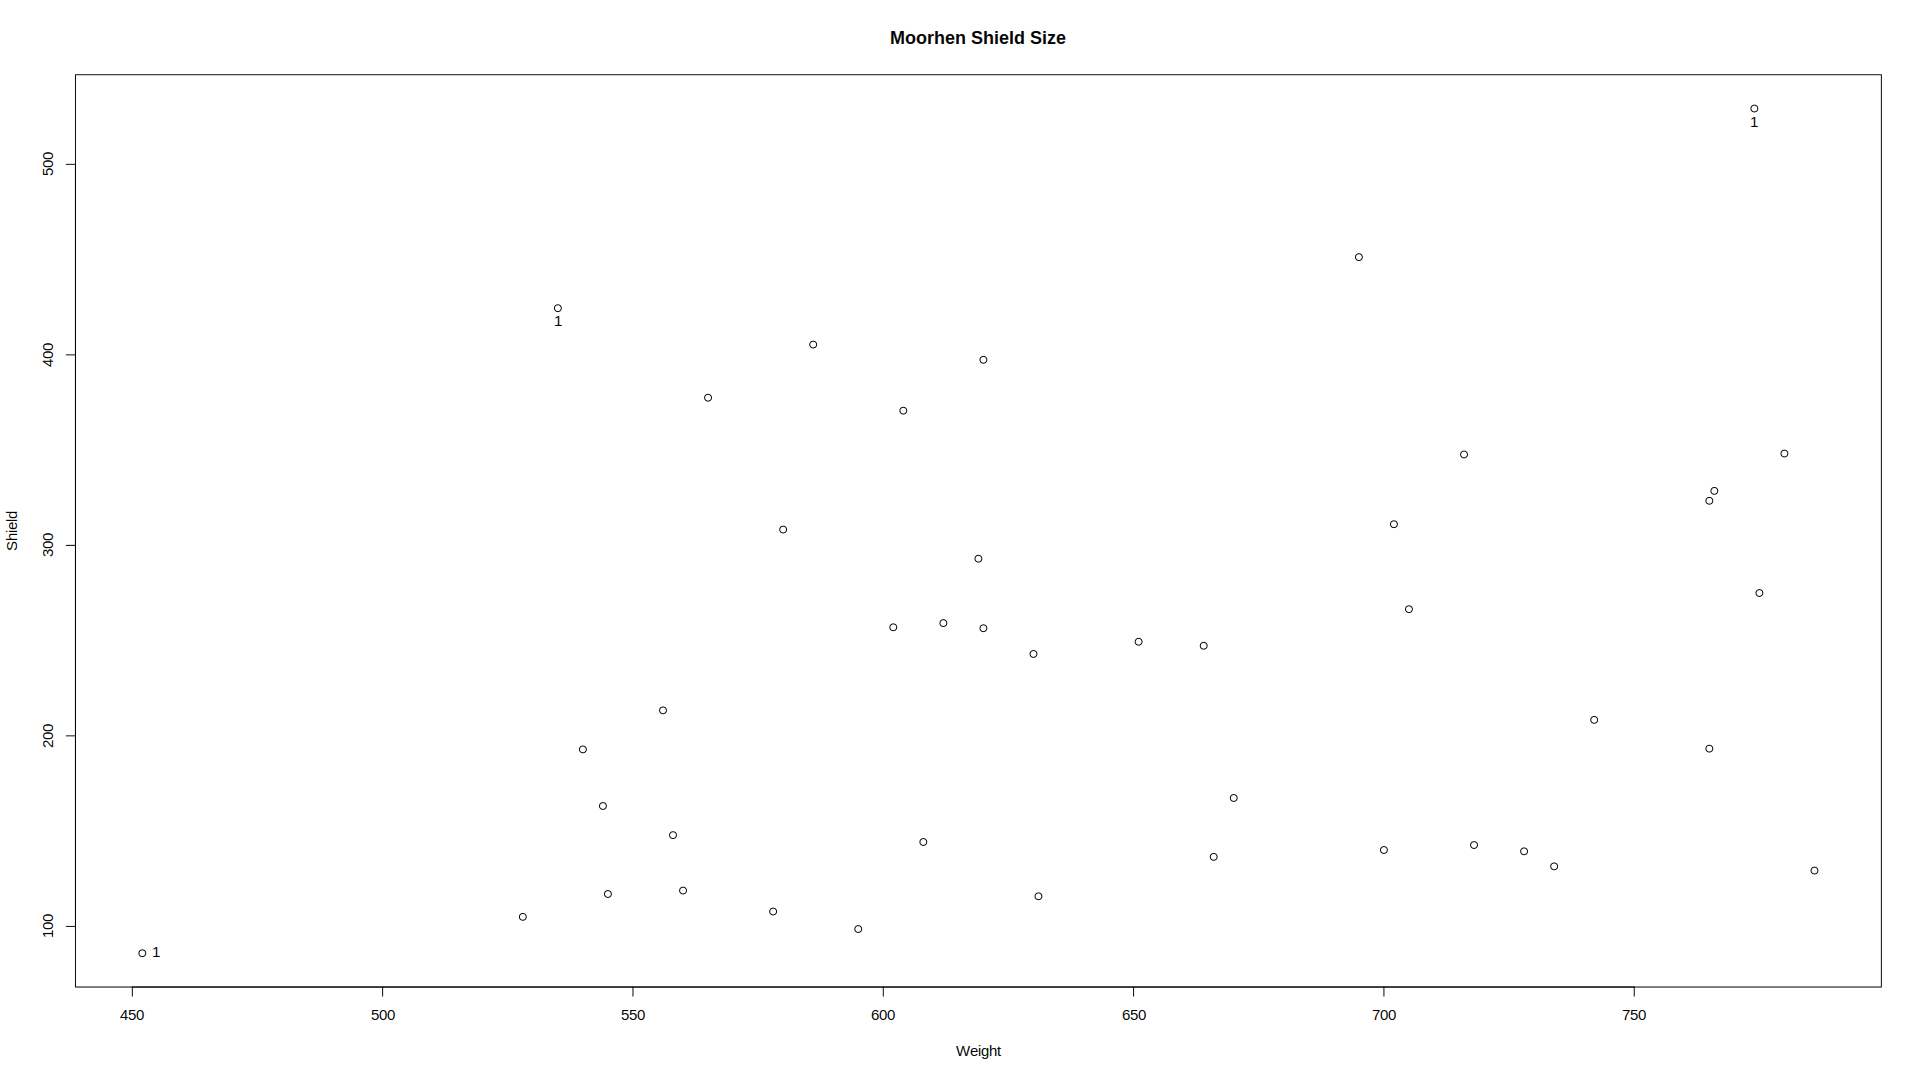
\includegraphics[width=\textwidth]{moorhen1}
  \caption{Plot with identified points}
  \label{fig:1}
\end{figure}

\begin{itemize}
\item Point \textbf{\textit{a}} was chosen because it is by far the lowest weight, and also one of the smallest shield sizes. This moorhen was most likely a juvenile.
\item Point \textbf{\textit{b}} shows a very large shield size for it's weight class, with larger shields only present in birds more than 100g heavier than this one in particular.
\item Point \textbf{\textit{c}} was one of the heavier birds, but exhibits the largest shield in the data.
\end{itemize}

\newpage

\subsection{}
\label{sec:1b}

Visually, there does not appear to be a strong correlation between shield size and weight, however some weak correlation could be argued for, as larger shields mostly show in higher weights. \\


\texttt{cor.test(Weight, Shield)} gives the following output:
\begin{verbatim}
t = 1.5793, df = 41, p-value = 0.122
alternative hypothesis: true correlation is not equal to 0
95 percent confidence interval:
 -0.06559203  0.50359325
sample estimates:
      cor 
0.2394694 
\end{verbatim}

Hypothesis test: $H_0:\rho = 0 $ vs $ H_A: \rho \neq 0$ \\
$t_{95}=1.58, p > 0.05$, so reject $H_A$, conclude that $\rho$ is not significantly different from 0. From the command output, we can see that the correlation is approximately 0.24, low enough to be disregarded.


\end{document}
